\input{$UNI_DIR/msc/tex/HWSetup}
\input{$UNI_DIR/msc/tex/EngBindings}

%
% Homework Details
%   - Title
%   - Subtitle
%   - Due date
%   - Due time
%   - Course
%   - Section/Time
%   - Instructor
%   - Author
%

\newcommand{\hmwkTitle}{HW00}
\newcommand{\hmwkSubTitle}{Homework Template}
\newcommand{\hmwkDueDate}{September 25th. 2025}
\newcommand{\hmwkDueTime}{09:30 AM}
\newcommand{\hmwkClass}{ENAE 441 - 0101}
\newcommand{\hmwkClassTime}{09:30 AM}
\newcommand{\hmwkClassInstructor}{Dr. Martin}
\newcommand{\hmwkAuthorName}{\textbf{Vai Srivastava}}
\newcommand{\hmwkCompletionDate}{\today}

\begin{document}

\maketitle

\pagebreak

\begin{hwkProblem}{1}{Parts}\label{hwk:p01}

	\begin{enumerate}
		\item \label{hwk:p01.01} Instructions
		\item \label{hwk:p01.02} Instructions
	\end{enumerate}

	\hwkSol{} \label{hwk:s01}

	\hwkPart{} \label{hwk:s01.01}

	Answer

	\hwkPart{} \label{hwk:s01.02}

	Answer

\end{hwkProblem}

\begin{hwkProblem}{2}{Code}\label{hwk:p02}

	Instructions

	\hwkSol{} \label{hwk:s02}

	\begin{figure}[H] \label{fig:s03}
		\begin{center}
			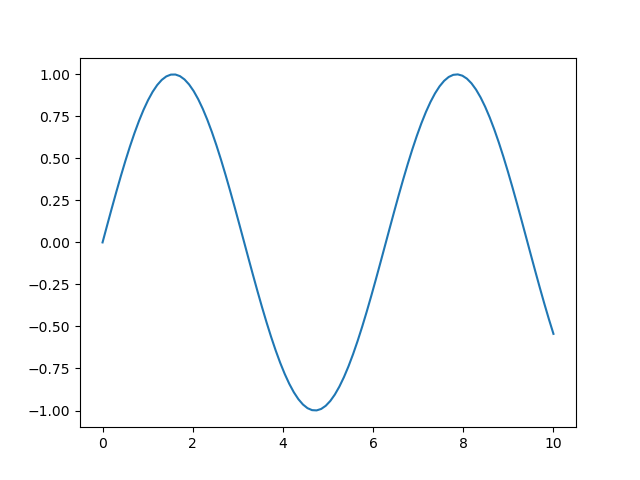
\includegraphics[width=0.95\textwidth]{./images/s03.png}
		\end{center}
		\caption{Example}
	\end{figure}

	\hwkCode{} \label{code:s02}

	See the \href{https://www.github.com/vaisriv/enae441-hw-template/blob/main/code/submission.py}{Python code} for this assignment.

\end{hwkProblem}

\end{document}
